%% 11. Identifying Bottlenecks

% Arithmetic intensity: FLOP vs. bandwidth limited
\begin{frame}[fragile]{Bottleneck Potpourri}

 \begin{block}{Arithmetic Intensity}
  \begin{itemize}
   \item Number of FLOPs per Byte
   \item FLOP-limited: AI larger than 1-10
   \item Memory-limited: AI smaller than 1-10
  \end{itemize}
 \end{block}

 \vspace*{-0.5cm}
 \begin{center}
   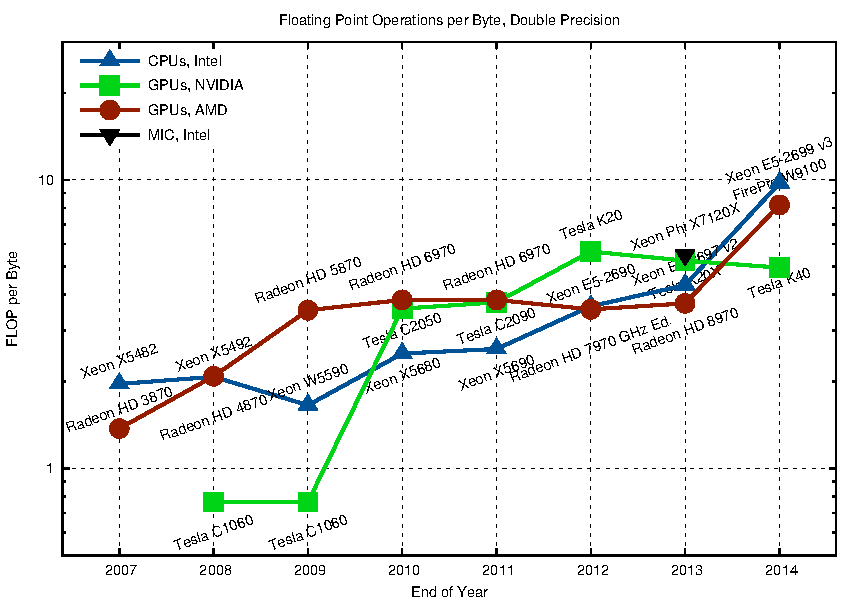
\includegraphics[width=0.7\textwidth]{figures/flop-per-byte-dp}
 \end{center}

\end{frame}


% 
% \begin{frame}[fragile]{Bottleneck Potpourri}
% 
%  \begin{block}{Arithmetic Intensity - Roofline Model}
%   \begin{itemize}
%    \item Determine maximum performance for given arithmetic intensity
%   \end{itemize}
%  \end{block}
% 
%  \begin{center}
%    \includegraphics[width=0.7\textwidth]{figures/roofline-1}
%  \end{center}
% 
% \end{frame}
% 
% 


% Latency

\begin{frame}[fragile]{Bottleneck Potpourri}

 \begin{block}{Latency}
  \begin{itemize}
   \item Bottleneck in strong scaling limit
   \item Ultimate limit for time stepping
  \end{itemize}
 \end{block}

 %\pause
 \begin{block}{Latency - Sources}
  \begin{itemize}
   \item Network latency (Ethernet $\sim 20 \mu$s, Infiniband $\sim 5 \mu$s)
   \item PCI-Express latency (Kernel launches, $\sim 10 \mu$s)
   \item Thread synchronization (barriers, locks, $\sim 1-10 \mu$s)
   \item Memory latency ($\sim 100$ns)
  \end{itemize}
 \end{block}

 \begin{center}
   \vspace*{-0.5cm}
   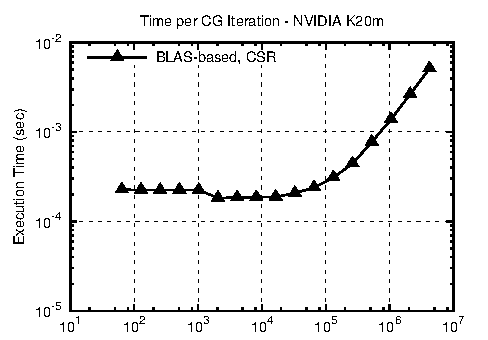
\includegraphics[width=0.4\textwidth]{figures/cg-k20m-0}
 \end{center}

\end{frame}



% Load imbalance

\begin{frame}[fragile]{Bottleneck Potpourri}

 \begin{block}{Load Imbalance}
  \begin{itemize}
   \item Total execution time determined by slowest thread
   \item Focus on making the slowest thread fast
   \item Easy for static data structures (e.g. dense matrices)
   \item Hard for dynamic data structures (e.g. sparse matrices)
  \end{itemize}
 \end{block}

%  \begin{center}
%    \includegraphics[width=0.7\textwidth]{figures/imbalance}
%  \end{center}

\end{frame}


% Amdahl's Law
\begin{frame}{Bottleneck Potpourri}
  \begin{block}{Amdahl's Law}
   \begin{itemize}
    \item $T_{\mathrm{total}} = T_{\mathrm{serial}} + T_{\mathrm{parallel}} / {\#\mathrm{processors}}$
    \item Speed-up limited by serial portion of an algorithm
   \end{itemize}
  \end{block}
  
%   \begin{center}
%    \includegraphics[width=0.7\textwidth]{figures/AmdahlsLaw}
%   \end{center}

\end{frame}